\section{Aufgabenstellung}

Sie setzen eine Lösung des bekannten Philosophenproblems um. Einzelne Teilnehmer, hier Philosophen, werden
in einzelnen Container realisiert. Diese kommunizieren ausschließlich mittels Nachrichten und die Zugriffe der
Teilnehmer werden verteilt koordiniert, d.h. keine (pseudo-) zentrale Lösung. Es sollen Performance-Messungen
für 5, 10 und eine von Ihnen zu ermittelnde maximal Anzahl von Container realisiert werden. Die RPC Lösung ist
hierbei komplett selbst zu erstellen und durch Tests abzusichern, bestehende Lösungen wie grpc, rmi, … sind nicht
zugelassen.

\begin{figure}[H]
\centering
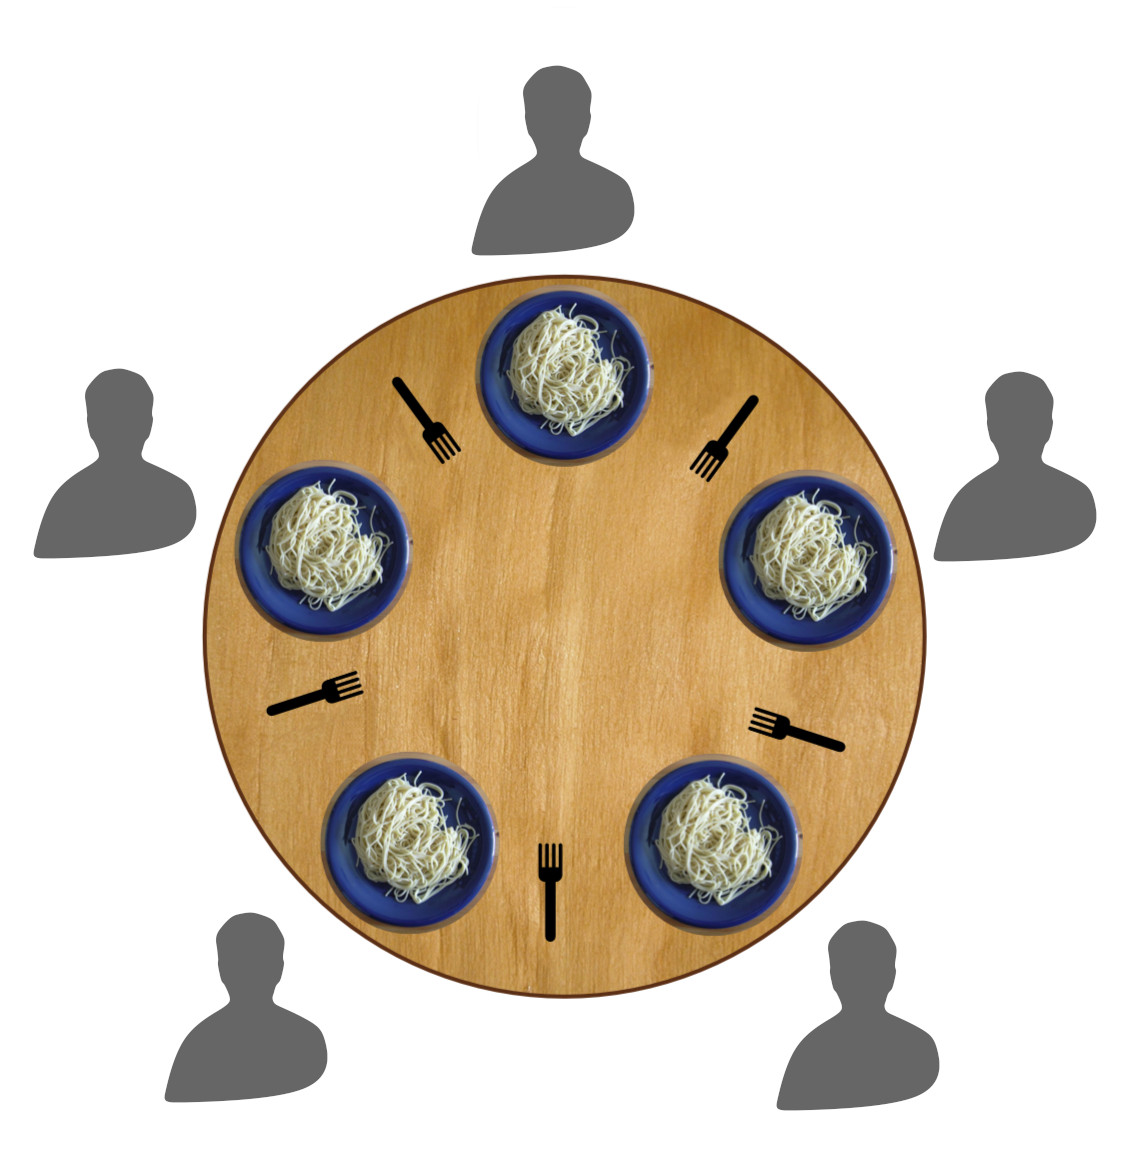
\includegraphics[width=0.7\textwidth]{images/Dining_philosophers_diagram.jpg}
\caption{Dining Philosophers}
\label{fig:DiningPhilosophers}
\end{figure}